\section{The saturation domain at the principal scale}\label{sec:main-saturation}
\label{sat:section}

The saturation domain has a limiting geometry described by a quartic with
four nonnegative roots. For a return with six fixed points, we first derive
the weights of the parameters and of the fixed points from the five
alternating extrema of its displacement. Estimates near the thresholds then
control critical points that
approach the thresholds, and their limiting values determine the four-root
region. The necessary estimates hold in every admissible family. We prove the
weights introduced in Section~\ref{sec:introduction}, beginning with
a tail estimate that converts weighted parameter bounds into bounds on the
fixed points.

\begin{lemma}[A tail bound from weighted parameters]\label{mainloc:tail}
For every fixed $K_0>0$, there are common constants $M,m_0>0$ such
that, whenever $0<|m|<m_0$ and
\[
 |a|\le K_0m^4,\qquad |b|\le K_0m^2,\qquad
 |\delta|\le K_0|m|^3,
\]
every zero of $D$ in $I$ satisfies $|q|<Mm^2$. On the two complementary
tails, $D$ has the sign of $c$.
\end{lemma}

\begin{proof}
Let $0<q_{\mathrm{in}}<q_0$ be an inner radius, to be fixed below.
For $Mm^2\le q\le q_{\mathrm{in}}$, reduce $m_0$ so that
$|\delta|/q\le K_0|m|/M\le1$. Equation~\eqref{eq:quartic-global-value}
gives
\[
 \frac{|Q-q|}{q^2}\le K\{M^{-1/2}+M^{-3/2}+m^2+\sqrt{q_{\mathrm{in}}}
                                      +m^2M^{-1/2}\}.
\]
In particular, the strength-sum and separation terms use respectively
$|m|/\sqrt q\le M^{-1/2}$ and
$|\delta|\sqrt{q+|\delta|}/q^2\le KM^{-3/2}$.
For small $q_{\mathrm{in}}$, this also gives $|Q-q|/q<1/2$. The closing
expansion yields
\[
 D-cq^2=a+bq+(1+b)(Q-q)
       +c\{2q(Q-q)+(Q-q)^2\}+Q^3S(Q,\lambda).
\]
Consequently
\begin{equation}\label{sat:tail-estimate}
 \frac{|D(q)-c(\lambda)q^2|}{q^2}
 \le K\{M^{-2}+M^{-1}+M^{-1/2}+M^{-3/2}
                              +\sqrt{q_{\mathrm{in}}}+|m|\}.
\end{equation}
The first two terms bound $a/q^2$ and $b/q$; the remaining closing
terms follow from $|Q|\le2q$ and the bound for $Q-q$.
For $-q_{\mathrm{in}}\le q\le-Mm^2$, both passage inputs are negative once $m_0$ is
small: $q<\min(0,\delta)$. Thus $Q=q$ exactly, and the same estimate
follows directly from the closing expansion. Choose $M$ large, then
$q_{\mathrm{in}}$ small and $m_0$ small so that the right-hand side is less than
half the common lower bound for $|c|$; reduce $m_0$ further so that
$Mm_0^2<q_{\mathrm{in}}$.

The rest of the original common interval $I=(-q_0,q_0)$ is covered as
follows. At the reference, \eqref{eq:center-displacement}
gives $D(0)=D'(0)=0$ and strict curvature of sign $c_0$ throughout
the reduced interval. Hence $D$ has that sign at every
nonzero reference state. The closed outer state set
$q_{\mathrm{in}}\le |q|\le q_0$ is compact and has a nonzero value margin; joint continuity in the
parameters preserves it after one common parameter reduction. The common domains are chosen to contain
$\overline I$, so this argument covers the whole interval.
All choices are made before any parameter path is chosen.
\end{proof}

\begin{lemma}[Returns with six fixed points]
\label{sat:saturation}\label{corner:saturated-geometry}
\label{cor:six-necessary-window}
If $D$ has six zeros in $I$, then
\[
 mc_0(p)<0,\qquad \delta A(p)c_0(p)<0,\qquad
 0<\delta/\delta_{\rm c}(m,p)<1.
\]
In particular $0<|\delta|<|\delta_{\rm c}|\le K|m|^3$ uniformly.
Put $s=-\sgn c_0$, $E=sD$, and denote the thresholds by $\theta_1<\theta_2$.
Then $P''$ has two simple zeros $\zeta_1<\zeta_2$ in the outer region, and
\begin{equation}\label{sat:curvature-signs}
 \begin{array}{c|ccccc}
 q&(-q_0,\theta_1)&(\theta_1,\theta_2)&(\theta_2,\zeta_1)&
       (\zeta_1,\zeta_2)&(\zeta_2,q_0)\\ \hline
 \sgn E''&-&+&-&+&-
 \end{array}
\end{equation}
The continuous $E'$ has exactly one zero in each open interval, none
at its shared junctions, and
\begin{equation}\label{sat:junction-slopes}
 E'(\theta_1)<0,\quad E'(\theta_2)>0,\quad
 E'(\zeta_1)<0,\quad E'(\zeta_2)>0.
\end{equation}
All six zeros are simple $C^1$ zeros, including any at a threshold.
The extremal values have signs $+,-,+,-,+$; the first is an inactive
positive maximum and the second a negative minimum between the thresholds.
On $\delta=\delta_{\rm c}$, $mc_0<0$, there are at most four fixed points.
\end{lemma}

\begin{proof}
The four-point slices exclude $m=0$ and $\delta=0$.
The signs~\eqref{eq:event-signs} give the number
$s_E=1+\mathbf1_{\{\delta Ac_0<0\}}$ of curvature sign changes at the thresholds.
Let $s_O\le2$ be the number of sign changes at zeros of $P''$ in the outer
region. Joining same-sign pieces through isolated zeros and thresholds gives at most $s_E+s_O+1\le5$
strict monotonicity blocks for the continuous $D'$. Each block,
with its finite endpoints, contains at most one zero. Six zeros of
$D$ give five distinct derivative zeros in their open gaps by $C^1$
Rolle, so $s_E=s_O=2$. Proposition~\ref{prop:cubic-curvature-window}
gives the stated window and cubic bound. The signs~\eqref{eq:event-signs} and the outer
factorization~\eqref{eq:curvature-factor} give~\eqref{sat:curvature-signs}.

Retain every shared finite junction in both adjacent blocks of $E'$.
A derivative zero there would occupy both blocks, leaving room for at
most four distinct derivative zeros. Hence all five lie in the five
respective interiors, and strict monotonicity gives
\eqref{sat:junction-slopes}. A stationary fixed point would supply a
sixth derivative zero distinct from the five open-gap zeros. Thus none
occurs, including at a threshold.
The extrema interlace the six roots, giving all five strict value signs.
At $\delta=\delta_{\rm c}$ the double zero of $P''$ does not change sign, leaving at most three blocks and four distinct fixed
points. Truncating at the ends of the common interval removes blocks
but cannot add them.
\end{proof}

\begin{proposition}[Weighted confinement]
\label{sat:weighted-confinement}
For every admissible family there are a further reduction of \(I\) and
\(U\) and a constant \(K>0\) with the following property. If \(P_\lambda\)
has six fixed points \(q_1,\ldots,q_6\) in \(I\), then
\begin{equation}\label{sat:weighted-bounds}
 0<|\delta|\le K|m|^3,\qquad
 |b|\le K|m|^2,\qquad |a|\le K|m|^4,\qquad
 \max_j|q_j|\le K|m|^2.
\end{equation}
\end{proposition}

\begin{proof}
We use the auxiliary-control convention following
Lemma~\ref{lem:auxiliary-controls} also when \(m\) and \(\delta\) are dependent.
The jets \(a,b\) are those of~\eqref{eq:regular-jets}.

Lemma~\ref{cor:six-necessary-window} already gives the first
bound in \eqref{sat:weighted-bounds}. At a curvature zero write
\(q=r^2\). The exact division \eqref{eq:V-division} gives
\begin{equation}\label{sat:curvature-state}
 \delta=r^2\{mH_\Delta(r,m,p)+rB_\Delta(r,p)\}.
\end{equation}
Here \(H_\Delta\) has sign \(A\), and \(B_\Delta\) has sign \(c_0/A\),
with uniform nonzero margins. In the sign case forced by six zeros,
\(mH_\Delta\) has the sign of \(\delta\), whereas \(rB_\Delta\) has the
opposite sign. Equation~\eqref{sat:curvature-state} consequently
implies
\begin{equation}\label{sat:curvature-scale}
 r\le K|m|,\qquad
 |v|=|\delta|/r^2=|mH_\Delta+rB_\Delta|\le K|m|
\end{equation}
at both zeros of \(P''\).

The derivative \(Q'\), taken at fixed parameters,
has the smooth root expression \eqref{eq:Q-outer}. It equals one
at \(r=0\), so \(Q'-1=rU_1(r,m,v,p)\) with \(U_1\) smooth.
The aligned strength cancellation gives \(U_1(0,0,0,p)=0\).
Hence
\begin{equation}\label{sat:outer-slope-bound}
 |Q'-1|\le K r(r+|m|+|v|).
\end{equation}
At \(\zeta_2\), equations~\eqref{sat:curvature-scale} and
\eqref{sat:outer-slope-bound}, together with \(Q=O(r^2)\), yield
\(D'(\zeta_2)=b+O(m^2)\). At the first threshold \(Q'=1\).
For positive separation that threshold is zero and \(Q=0\), giving
\(D'(\theta_1)=b\); for negative separation it is \(\delta\), with
\(Q=\delta\), giving \(D'(\theta_1)=b+O(|\delta|)\).
The first and last inequalities in \eqref{sat:junction-slopes}
therefore imply
\[
 -Km^2\le sb\le K|\delta|.
\]
The cubic separation bound proves \(|b|\le K|m|^2\).

For the offset and the states, use the bound
\eqref{eq:quartic-global-value}, which is uniform up to the thresholds.

On the inactive side the exact closing expansion gives
\[
 E(q)=sa+sbq+sc(\lambda)q^2+O(|q|^3).
\]
After shrinking the state interval, its last two terms are bounded
above by \(-\gamma q^2\) for one \(\gamma>0\). Completing the
square gives \(E(q)\le sa+Kb^2\). The positive inactive maximum
from Lemma~\ref{sat:saturation} therefore implies
\begin{equation}\label{sat:offset-lower-coarse}
 sa\ge-Kb^2.
\end{equation}
The next, negative minimum lies between the two thresholds, where
\(|q|\le K|\delta|\). Equation~\eqref{eq:quartic-global-value} and the
closing expansion give there
\[
 |D(q)-a|\le K\{ |b\delta|+|\delta|^{3/2}+\delta^2\}.
\]
Consequently
\begin{equation}\label{sat:offset-upper-coarse}
 sa\le K\{ |b\delta|+|\delta|^{3/2}+\delta^2\}
       \le K|m|^{9/2}.
\end{equation}
Together with \eqref{sat:offset-lower-coarse}, this proves
\(|a|\le K|m|^4\).

The three parameter bounds just proved satisfy the hypotheses of
Lemma~\ref{mainloc:tail}, which confines every zero to $|q|<Mm^2$.
\end{proof}

\subsection{The four-root limit}\label{subsec:four-root-limit}

The parameter and state weights are now forced by the six-point
configuration. We next identify the coefficient geometry of its limits.

Fix the sign case $A_1(\lambda_0)=B>0$ and $c_0=-C<0$, and define
\[
 A_4=C^3a/m^4,\qquad S_4=-Cb/m^2,\qquad
 T_4=3BC^2\delta/(2m^3),\qquad x=C\sqrt q/m.
\]
Here $B$ and $C$ are reference values. Write
\[
 \Phi_{A,S,T}(x)=A-Sx^2+x^3-x^4+Tx,
 \qquad
 \mathcal K_4=\{(-e_4(r),e_2(r),e_3(r)):r_i\ge0,\ \sum_i r_i=1\}.
\]

Let $\Lambda$ be the standard unfolding, defined on a neighbourhood
$\mathcal V\subset\mathbb R^4$ of $0$. Write
\[
 N_\lambda(I)=\#\{q\in I:D_\lambda(q)=0\},\qquad
 v_m(A,S,T)=\left(\frac{m^4A}{C^3},-\frac{m^2S}{C},m,
                         \frac{2m^3T}{3BC^2}\right).
\]
Choose a compact box $\mathcal B$, independent of $m$, containing
$\mathcal K_4$ in its interior and the normalized parameters of every
six-cycle configuration in $\mathcal V$;
Proposition~\ref{sat:weighted-confinement} provides such a box after
shrinking $\mathcal V$. Define
\begin{equation}\label{def:actual-main-domain}
 \mathscr T_m=\{(A,S,T)\in\mathcal B:v_m(A,S,T)\in\mathcal V,
                    N_{\Lambda(v_m(A,S,T))}(I)=6\}.
\end{equation}

For $x>0$ put $F_m(x)=C^3m^{-4}D(m^2x^2/C^2)$. At fixed parameters,
\[
 D_q=\frac{m^2}{2Cx}F_m',\qquad
 D_{qq}=\frac{C}{4x^3}(xF_m''-F_m').
\]
Thus the limiting curvature equation is
$x\Phi''-\Phi'=3x^2-8x^3-T=0$, with positive critical point $x=1/4$,
critical value $T=1/16$, and nonzero root $x=3/8$ when $T=0$.

\begin{lemma}[Convergence at the principal scale]\label{lem:k4-sequence}
Let parameters tend to the reference, let $m>0$ tend to zero, and assume
that $(A_4,S_4,T_4)$ stays bounded. If these triples converge to $(A,S,T)$,
then
\[
 \frac{C^3}{m^4}D(m^2x^2/C^2)\longrightarrow\Phi_{A,S,T}(x)
\]
in $C^k$ on every compact subset of $x>0$, for every fixed finite $k$.
\end{lemma}
\begin{proof}
Put $r=mx/C$ and $v=\delta/r^2=2mT_4/(3Bx^2)$. On a positive compact
$x$-interval, $r,m,v\to0$ uniformly with all fixed-order $x$ derivatives.
The division~\eqref{eq:actual-both-active-division} gives
\[
 Q-q=mr^3+\tfrac34m^2r^4+r^5L_0+\delta rH,
 \qquad H(0,0,0,p)=\tfrac32A_1(p,0,0).
\]
Consequently $C^3(Q-q)/m^4\to x^3+Tx$ in every such $C^k$ norm.
In the closing expansion
\[
 D=a+bQ+(Q-q)+c(\lambda)Q^2+Q^3S_R,
\]
we have $Q=q+O_{C^k}(m^4)$, $b=-m^2S_4/C$, and $c(\lambda)\to-C$.
The four remaining terms therefore converge respectively to
$A$, $-Sx^2$, $-x^4$, and zero after multiplication by $C^3/m^4$.
All profiles are evaluated in one compact neighbourhood, so their state
derivatives are controlled however the remaining parameters converge.
\end{proof}

Convergence on positive compact intervals leaves open the behaviour near
the thresholds. The next lemma controls the critical point that can collapse
onto a threshold.

\begin{lemma}[Critical points near the thresholds]\label{lem:k4-event}
Let parameters tend to the reference through returns with six fixed points,
and let their normalized coefficients converge to $(A,S,T)$. Denote the five successive critical points of $D$
by $t_1,\ldots,t_5$, and put $x_j=C\sqrt{t_j}/m$ for $j=3,4,5$.
If $T>0$, all three $x_j$ stay in a compact subset of $(0,\infty)$.
If $T=0$, then $x_3\to0$, $A=0$, and every limit of $x_5$ is at least
$3/8$.
\end{lemma}
\begin{proof}
The critical points interlace the six zeros, so their upper bounds follow
from the state confinement in \eqref{sat:weighted-bounds}. The offset
estimate~\eqref{sat:offset-upper-coarse} gives
$a\le K m^{9/2}$, hence $A\le0$.

Suppose first that $T>0$ and that $x_3\to0$ along a subsequence.
At $q=t_3$ both passages are active. Let $y=\Gamma_1(q)-\delta\ge0$.
Since $q^{3/2}/\delta$ is a fixed positive constant times $x_3^3/T_4$,
this ratio tends to zero. More generally, on the common small parameter
and state domain, assume $A_1\ge B/2$, $m>0$, $\delta>0$, $q>0$ and
$y\ge0$. If $q^{3/2}/\delta$ is sufficiently small, the passage value
estimate gives
\[
 q-y\ge\delta/2,\quad 0\le y<q,\quad
 \sqrt q-\sqrt y\ge\delta/(4\sqrt q).
\]
The derivative expansion, with all coefficients evaluated at the same
parameter, is
\[
 Q_q-1=\tfrac32A_1(\sqrt q-\sqrt y)
       +\tfrac32(A_1+A_2)\sqrt y+O(q).
\]
The strength identity gives $A_1+A_2=m>0$. Also $Q=O(q)$,
$Q_q=1+O(\sqrt q)$, and $R'(Q)-1=b+O(q)$. Consequently, for common
constants $\kappa,K>0$,
\begin{equation}\label{sat:threshold-slope-exclusion}
 D_q(q)\ge \kappa\delta/\sqrt q-K(|b|+q).
\end{equation}
This estimate includes $y=0$, the second threshold, by continuity of the
passage derivatives. Applied at $t_3$ and multiplied by $C/m^2$, its
right-hand side is bounded below by
$\kappa_1T_4/x_3-K_1-K_2x_3^2$, which tends to $+\infty$. This contradicts
$D_q(t_3)=0$. The ordering $x_3<x_4<x_5$ proves the first assertion.

Now suppose $T=0$. Write $r_-<r_+$ for the square roots of the two zeros
of $P''$ in the outer region. They lie on opposite sides of the unique
positive critical point $r_{\rm c}$ of the separation graph. Its exact
formula~\eqref{sat:curvature-state} and the boundary coefficients in
\eqref{eq:B-boundary}--\eqref{eq:V-division} give, for bounded $x=Cr/m$,
\[
 T_4=3x^2-8x^3+o(1),\qquad Cr_{\rm c}/m\longrightarrow1/4.
\]
The error is uniform down to $x=0$ because the graph profiles are smooth.
Both $Cr_\pm/m$ are bounded by the curvature-zero confinement
\eqref{sat:curvature-scale}. A limit
of $Cr_-/m$ lies in $[0,1/4]$ and solves $x^2(3-8x)=0$, hence is zero.
A limit of $Cr_+/m$ is at least $1/4$ and solves the same equation, hence
is $3/8$. Since $t_3<r_-^2$ and $t_5>r_+^2$, the location assertions follow.

The estimate~\eqref{eq:quartic-global-value} yields
\[
 |D(q)-a|\le K\{|b|q+q^2+mq^{3/2}+m^2q^2+q^{5/2}
                +\delta\sqrt{q+\delta}+\delta q^{3/2}\}.
\]
At $q=t_3$, division by $m^4$ bounds this by a constant times
\[
 x_3^2+x_3^3+x_3^4+m^2x_3^4+mx_3^5
 +T_4x_3+\sqrt m\,T_4^{3/2}+m^2T_4x_3^3,
\]
which tends to zero. Since $D(t_3)>0$, this gives $A\ge0$, and therefore
$A=0$.
\end{proof}

These two convergence statements allow the critical-value signs to pass
to the quartic, including its zero-root face.

\begin{proposition}[Necessary four-root geometry]\label{prop:k4-necessary}
In this sign case, for every admissible family, every accumulation point of
$(A_4,S_4,T_4)$ along a saturated sequence belongs to $\mathcal K_4$.
\end{proposition}
\begin{proof}
Take a convergent coefficient subsequence, using \eqref{sat:weighted-bounds}.
In this sign case \eqref{sat:junction-slopes} gives $b=D'(0)<0$ on every
saturated return, so $S_4=-Cb/m^2>0$ and its limit satisfies $S\ge0$.
If $T>0$, Lemmas~\ref{lem:k4-sequence} and~\ref{lem:k4-event} give three
positive limiting critical points $u\le v\le w$ of $\Phi$, with
\[
 \Phi(u)\ge0,\qquad\Phi(v)\le0,\qquad\Phi(w)\ge0.
\]
If $k\le3$ critical points converge to the same positive point $z$,
repeated Rolle gives zeros of $F_m^{(j)}$ tending to $z$ for
$1\le j\le k$. The $C^3$ convergence yields $\Phi^{(j)}(z)=0$ for
those $j$, so $z$ is a zero of $\Phi'$ of multiplicity at least $k$.
If $u<v<w$, the four successive intervals
$[0,u],[u,v],[v,w],[w,\infty)$ each contain a zero, since $\Phi(0)=A\le0$
and $\Phi$ tends to $-\infty$. A zero at a shared critical endpoint has
multiplicity at least two, so the four interval allocations are valid
when counted with multiplicity. If $u=v<w$, then $\Phi(u)=0$ and the
double derivative zero gives a triple polynomial zero at $u$; a fourth
zero lies in $[w,\infty)$. The case $u<v=w$ is analogous. If all three
merge, the common value is zero and the root has multiplicity four.
Thus all four roots are nonnegative and their sum is one.

If $T=0$, Lemma~\ref{lem:k4-event} gives $A=0$. After subselection $x_5\to w\ge3/8$,
and positive-compact convergence gives $\Phi(w)\ge0$. Therefore
$-S+w-w^2\ge0$, so $0\le S\le1/4$. The factorization
$\Phi=x^2(-x^2+x-S)$ again gives four nonnegative roots with sum one.
\end{proof}

\begin{proof}[Completion of Theorem~\ref{thm:main-saturation-summary}]
The interior of $\mathcal K_4$ consists exactly of coefficient triples
with four distinct positive roots. The set of such triples is open by simple-root
continuation. A zero root or a multiple root is a boundary point: a
small constant-term perturbation gives respectively a negative root or
violates one of the necessary critical-value signs for four real roots.
Triples with distinct positive roots are dense, by perturbing the root
vector inside the simplex while preserving its sum.

For positive roots $r_i$ of an interior triple, the construction in the
proof of Proposition~\ref{prop:single-scale-six} with $r_i/C$ and $\eps=m$
gives exactly the parameters $v_m(A,S,T)$ and two simple negative roots. On
each compact subset of the interior, uniform isolation and nonzero derivative
margins let Lemma~\ref{lem:weighted-quartic} continue all six roots in the
standard unfolding for uniformly small $m>0$; Proposition~\ref{prop:common-count}
excludes others in $I$.

For the Hausdorff upper inclusion, a contrary sequence of closure points
can be approximated within $1/n$ by true points of $\mathscr T_{m_n}$.
Compactness of $\mathcal B$ and Proposition~\ref{prop:k4-necessary} then
force its limit into $\mathcal K_4$. For the lower inclusion, approximate
compact $\mathcal K_4$ by a finite net of interior points and realize all
of them at every sufficiently small $m$.
\end{proof}

\subsection{Boundary geometry of the limiting domain}

Figure~\ref{fig:main-saturation-sections} displays two sections of the
limiting coefficient region; the critical-value criterion below describes
their boundaries.

\begin{figure}[!htbp]
\centering
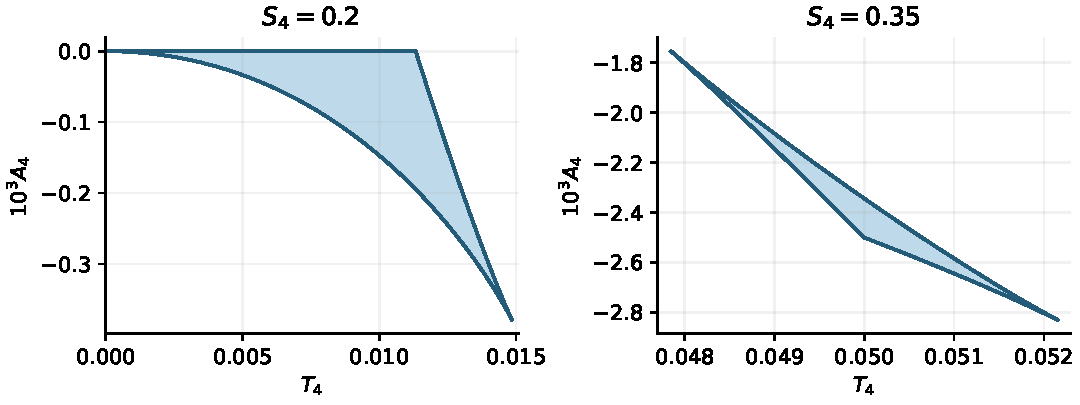
\includegraphics[width=\textwidth]{figures/main-saturation-sections.pdf}
\caption{Sections of the limiting four-root domain at $S_4=0.2$ and
$S_4=0.35$. The ordinate is $10^3A_4$, and the two panels have different
axis ranges. The boundaries are drawn from the critical-value interval
described below. In the left panel the segment $A_4=0$ represents a zero
root. The remaining boundary arcs have repeated roots; the two lower
bounds switch when $f(u)=f(w)$, where the two local maxima have equal value.}
\label{fig:main-saturation-sections}
\end{figure}

The symmetric mean inequalities give
\[
 -\frac1{256}\le A_4\le0,\qquad
 0\le S_4\le\frac38,\qquad 0\le T_4\le\frac1{16}.
\]
The three coefficient extrema $A_4=-1/256$, $S_4=3/8$,
and $T_4=1/16$ are attained at $r_i=1/4$, where
$\Phi=-(x-1/4)^4$. At the opposite face, $e_3=0$ forces at least two
roots to vanish, and therefore
\[
 \mathcal K_4\cap\{T_4=0\}
 =\{(0,S_4,0):0\le S_4\le1/4\}.
\]
These bounds are sharp for $\mathcal K_4$ and hold asymptotically along
saturated sequences.

For fixed $S_4,T_4$ with three positive critical points $u<v<w$, put
$f(x)=-S_4x^2+x^3-x^4+T_4x$. The admissible offset interval is
\[
 \max\{-f(u),-f(w)\}\le A_4\le\min\{0,-f(v)\}.
\]
It is nonempty precisely when these critical-value inequalities are
compatible. Taking closures includes merged critical points in this
description of the limiting boundary.
